% SSEE — Unified Journal Paper
% Target: JCAP / PRD / Universe (MDPI)
% Compile: pdflatex (×2) + bibtex + pdflatex (×2)
\documentclass[12pt,a4paper]{article}

\usepackage[utf8]{inputenc}
\usepackage{amsmath,amssymb,amsfonts}
\usepackage{graphicx}
\usepackage{booktabs}
\usepackage[colorlinks=true,linkcolor=red!70!black,citecolor=green!50!black,urlcolor=blue!80!black]{hyperref}
\usepackage{xcolor}
\usepackage{geometry}
\usepackage{natbib}
\usepackage{caption}
\usepackage{float}
\usepackage{array}
\usepackage{tabularx}
\usepackage{enumitem}
\usepackage{tcolorbox}
\usepackage{multirow}
\geometry{margin=2.5cm}
\emergencystretch=2em

% ─── Macros ──────────────────────────────────────────────────────────────────
\newcommand{\SSEE}{\textsc{ssee}}
\newcommand{\LCDM}{$\Lambda$CDM}
\newcommand{\phiG}{\varphi}
\newcommand{\KAL}{\mathrm{KAL}_0}
\newcommand{\MIRA}{\mathcal{M}}
\newcommand{\AURA}{\mathrm{AURA}}
\newcommand{\thetaE}{\theta_E}
\newcommand{\fscr}{f_{\mathrm{scr}}}
\newcommand{\Omde}{\Omega_{\mathrm{DE}}}
\newcommand{\Omm}{\Omega_{m}}
% 2026-09-26: era \newcommand{\sm}{\Omega_{m,\mathrm{dyn}}}. El nombre del
% macro decia «densidad de materia» de un numero que es $1+w_0$, y la prosa
% de abajo lo repetia. Pasa a $s_m$, el simbolo que ya usan Papers 1, 7 y 10.
\newcommand{\sm}{s_m}
\newcommand{\OmmCMB}{\Omega_{m,\mathrm{CMB}}}
\newcommand{\wz}{w_0}
\newcommand{\wa}{w_a}
\newcommand{\sig}{\sigma_8}
\newcommand{\sigeff}{\sigma_8^{\mathrm{eff}}}
\newcommand{\kfs}{k_{\mathrm{fs}}}
\newcommand{\mphi}{m_\phi}
\newcommand{\fsig}{f\sigma_8}
\newcommand{\alphaK}{\alpha_K}
\newcommand{\alphaB}{\alpha_B}
\newcommand{\alphaM}{\alpha_M}
\newcommand{\alphaT}{\alpha_T}
\newcommand{\half}{\tfrac{1}{2}}
\newcommand{\GR}{\mathrm{GR}}

% ─────────────────────────────────────────────────────────────────────────────
\title{\textbf{Structural Self-Energy Expansion (SSEE):\\
A Minimal-Parameter Dark Energy Framework ---\\
Algebraic Derivation, Boltzmann Validation, and\\
Effective Field Theory Stability Analysis}}

\author{Mike Edison Almeida Vallejo \\
\small \textit{Independent Researcher} \\
\small \href{mailto:mike.almeida1721@gmail.com}{mike.almeida1721@gmail.com} \\
\small ORCID: \href{https://orcid.org/0009-0008-2195-7836}{0009-0008-2195-7836}
}

\date{May 2026}

% ─────────────────────────────────────────────────────────────────────────────
\sloppy
% ACTA-PROCEDENCIA {"commit": "5651fc97a90dc17d52be0317b46142db9ac86fcb", "reproducible_desde_commit": true, "cambios_sin_commitear": [], "script": "src/valores_tex.py", "script_sha256": "cb5ceb2369bdef5e586d471d57d44a11a9fed354be540a96ce34da85e582efa4", "nucleo_sha256": "5cec8af72d88f154116c5a532e42a9b6ff7a5b4c3d86bcc6921eabb246698993", "entradas": {"manuscript/valores.yaml": "5fa01e91dd68164243d664a73264bb6c87431d2ec0bd69db87c62a983a55992d", "results/logs/kids_publicados.json": "6c25c98059ce91038215358b4e7ac9cfb40198f410354937cee4ea00b46654ff", "results/logs/p10_uv_fscreen.json": "8fb68b295c848e0292e5701e7de795ba7c7ba25e3292d776260bb3dea8970c95", "results/logs/s8_desde_b1.json": "6d225f4403fbfbe6934d7edca26aaefbbe19e05ef6c7b7eda842a259e798b1c1"}, "argv": ["src/valores_tex.py"], "fecha": "2026-09-30T19:35:24", "host": "mike-System-Product-Name", "python": "3.12.3", "versiones": {}, "nucleos": {"OMP_NUM_THREADS": null, "MKL_NUM_THREADS": null, "OPENBLAS_NUM_THREADS": null, "OMPI_COMM_WORLD_SIZE": null}}
% GENERADO por src/valores_tex.py desde manuscript/valores.yaml — NO EDITAR A MANO.
% Cada numero sale de un log de la cadena de procedencia (dvc.yaml + acta).
\providecommand{\val}[1]{\csname ssee@val@#1\endcsname}
\expandafter\def\csname ssee@val@H0_glob\endcsname{67.962142}  % results/logs/p10_uv_fscreen.json#H0_glob
\expandafter\def\csname ssee@val@PTE_k1000_lcdm\endcsname{0.010}  % results/logs/kids_publicados.json#PTE.lcdm.PTE
\expandafter\def\csname ssee@val@PTE_k1000_ssee\endcsname{0.012}  % results/logs/kids_publicados.json#PTE.ssee.PTE
\expandafter\def\csname ssee@val@S8_b1_lcdm\endcsname{0.8229}  % results/logs/s8_desde_b1.json#filas.LCDM.S8
\expandafter\def\csname ssee@val@S8_b1_lcdm_sigma\endcsname{0.0059}  % results/logs/s8_desde_b1.json#filas.LCDM.S8_sigma
\expandafter\def\csname ssee@val@S8_b1_ssee\endcsname{0.8261}  % results/logs/s8_desde_b1.json#filas.SSEE.S8
\expandafter\def\csname ssee@val@S8_b1_ssee_sigma\endcsname{0.0054}  % results/logs/s8_desde_b1.json#filas.SSEE.S8_sigma
\expandafter\def\csname ssee@val@S8_legacy_dato\endcsname{0.8265}  % results/logs/kids_publicados.json#kids_legacy.S8
\expandafter\def\csname ssee@val@S8_legacy_dato_sigma\endcsname{0.0176}  % results/logs/kids_publicados.json#kids_legacy.S8_sigma
\expandafter\def\csname ssee@val@chi2_k1000_lcdm\endcsname{262.75}  % results/logs/kids_publicados.json#PTE.lcdm.chi2
\expandafter\def\csname ssee@val@chi2_k1000_publicado\endcsname{260.31}  % results/logs/kids_publicados.json#kids1000_maxpost.chi2
\expandafter\def\csname ssee@val@chi2_k1000_ssee\endcsname{265.44}  % results/logs/kids_publicados.json#PTE.ssee.chi2
\expandafter\def\csname ssee@val@dAIC_k1000\endcsname{-5.31}  % results/logs/kids_publicados.json#seleccion_kids1000.delta_AIC
\expandafter\def\csname ssee@val@dBIC_k1000\endcsname{-19.0}  % results/logs/kids_publicados.json#seleccion_kids1000.delta_BIC
\expandafter\def\csname ssee@val@dchi2_k1000\endcsname{2.69}  % results/logs/kids_publicados.json#seleccion_kids1000.delta_chi2
\expandafter\def\csname ssee@val@fscreen_IR\endcsname{0.067253}  % results/logs/p10_uv_fscreen.json#f_screen_IR
\expandafter\def\csname ssee@val@fscreen_UV_corr\endcsname{0.002268}  % results/logs/p10_uv_fscreen.json#f_screen_UV_corr
\expandafter\def\csname ssee@val@fscreen_full\endcsname{0.069522}  % results/logs/p10_uv_fscreen.json#f_screen_full
\expandafter\def\csname ssee@val@logA_b1_lcdm\endcsname{3.045}  % results/logs/s8_desde_b1.json#filas.LCDM.logA
\expandafter\def\csname ssee@val@logA_b1_ssee\endcsname{3.042}  % results/logs/s8_desde_b1.json#filas.SSEE.logA
\expandafter\def\csname ssee@val@logA_b1_ssee_sigma\endcsname{0.013}  % results/logs/s8_desde_b1.json#filas.SSEE.logA_sigma
\expandafter\def\csname ssee@val@p_dchi2_k1000\endcsname{0.61}  % results/logs/kids_publicados.json#seleccion_kids1000.p_delta_chi2
\expandafter\def\csname ssee@val@sK_IR\endcsname{0.403302}  % results/logs/p10_uv_fscreen.json#s_K_IR
\expandafter\def\csname ssee@val@sK_UV_corr\endcsname{0.013603}  % results/logs/p10_uv_fscreen.json#s_K_UV_corr
\expandafter\def\csname ssee@val@sK_full\endcsname{0.416905}  % results/logs/p10_uv_fscreen.json#s_K_full
\expandafter\def\csname ssee@val@tension_b1_lcdm\endcsname{2.59}  % results/logs/s8_desde_b1.json#filas.LCDM.tension_kids
\expandafter\def\csname ssee@val@tension_b1_ssee\endcsname{2.73}  % results/logs/s8_desde_b1.json#filas.SSEE.tension_kids
\expandafter\def\csname ssee@val@z_k1000_lcdm\endcsname{2.5}  % results/logs/kids_publicados.json#PTE.lcdm.z
\expandafter\def\csname ssee@val@z_k1000_ssee\endcsname{2.4}  % results/logs/kids_publicados.json#PTE.ssee.z

\begin{document}

\maketitle

% ─── Abstract ────────────────────────────────────────────────────────────────
\begin{abstract}
We present the Structural Self-Energy Expansion (\SSEE), a dark energy
framework that derives its cosmological background sector algebraically
from the golden ratio $\phiG$ and $\pi$, with zero fitted dimensionless
parameters at the background level and no WIMP, QCD-axion, or SUSY dark-matter
particle. Phenomenological extensions in the dark-matter sector, proposed in an
earlier version of Paper~6, are \emph{retracted} (\S\ref{sec:growth_raw}): the
matter sector is a single unpartitioned component, and their register entries
(OP-9, OP-11) close by dissolution (\texttt{OPEN\_PROBLEMS.md}). In CMB-likelihood terms SSEE is a $k=2$ fit: of
$\Lambda$CDM's six parameters it fixes four algebraically ($\Omega_b$, $\Omega_c$
via $\omega_c=\mathrm{KAL}_0\,\omega_b\,n_s$, $n_s=1-\phiG^{-7}$, and the derived
anchor $H_0/(\mathrm{km\,s^{-1}\,Mpc^{-1}})=3(\phiG+\pi)^2$), leaving only the primordial amplitude $A_s$ and the
optical depth $\tau$ ($k=2$ versus $k=6$, the count used in the Paper~3 model
comparison).
The dark energy equation of state $\wz = -(3\phiG+\pi)/[2(\phiG+\pi)] \simeq -0.840$
and $\wa \simeq -0.670$ are fixed by the algebraic construction and agree with the
official DESI~DR2 $w_0w_a$CDM posterior within $0.24\sigma$ (Pantheon+;
$0.2$--$1.8\sigma$ across SN compilations)---a parameter-free postdiction, with no
claim of temporal priority over DESI~DR2.
A Bayesian MCMC analysis under the global rate $H_0^{\rm glob}$ as prior
($H_0^{\rm prior,SSEE}=H_0^{\rm glob}=H_{\rm SH0ES}(1-f_{\rm screen})=\val{H0_GLOBAL_d3}\pm0.968$~km\,s$^{-1}$\,Mpc$^{-1}$, which is also
the value at which Planck~\texttt{plik\_lite} is minimised with SSEE-fixed $\omega_b,\omega_c$; Papers~3, 9--10) yields
$H_0 = 67.82^{+0.41}_{-0.41}$~km\,s$^{-1}$\,Mpc$^{-1}$ ($0.68\sigma$ from Planck,
$0.33\sigma$ from $H_0^{\rm glob}$) and $\Delta\mathrm{BIC}=\val{p2_dBIC_lcdm}$ favouring
\SSEE\ over \LCDM\ ($\val{p2_dBIC_cpl}$ over CPL).
A complementary full-likelihood multi-probe MCMC (CAMB $+$ Planck
\texttt{plik\_lite} $+$ lensing $+$ DESI~DR2 $+$ $f\sigma_8$, $w_0,w_a$ free and
$H_0$ under a flat prior) places the model at $1.31\sigma$ in the $w_0$--$w_a$
plane, where \LCDM\ is excluded at $3.22\sigma$; under this uncompressed CMB
likelihood $H_0$ relaxes to $65.87\pm1.17$ ($1.79\sigma$ below the anchor).

The CMB-sector matter density is the standard physical observable
$\OmmCMB = \omega_m/h^2 = \val{OMEGA_M_TOTAL_d6}$ (Planck: $0.3153\pm 0.0073$), built
piece-by-piece from SSEE algebra ($\omega_m$-direct; OP-8 dissolved, no matter
factor) and distinct from the saturation $\sm = 1+w_0 = \val{S_M_d6}$, which fixes
the DESI BAO equation of state and is not a density at all.
Full-sky CLASS Boltzmann runs confirm that the \emph{full} matter density is
physically necessary: using only $\sm=\val{S_M_d6}$ as the CMB matter density
shifts the peak positions by $\sim 10\%$ and raises the RMS residual
from $\val{cl_ssee_rms}\%$ to $\val{cl_naive_rms}\%$.

A linear Israel-Stewart perturbation analysis with $\Omega_{m,\mathrm{cosm}}=\val{OMEGA_M_TOTAL_d6}$ in
the Poisson equation yields a growth factor
$\mathcal{G} = 1.0032$ and $\sigma_8 = 0.8136$ (Paper~5), giving a mean
$\fsig$ tension of $0.70\sigma$ across six RSD surveys --- statistically identical
to $\Lambda$CDM ($0.73\sigma$), resolving the growth-rate sector.
In the lensing amplitude, against the $357$ \emph{raw} \textsc{KiDS-Legacy}
$\xi_\pm$ points, with a \emph{single} unpartitioned matter sector, the
background fixed by the algebra and $A_s$ fixed to the value the model's own
CMB fit supplies --- \emph{no} free cosmological parameter --- the model predicts
$S_8=0.8273$ against $0.8265\pm0.0176$ measured
($0.05\sigma$).\footnote{Updated 2026-09-26. KiDS-Legacy (Wright et al.\ 2025,
arXiv:2503.19441) was published sixteen months before this analysis; no temporal
priority is claimed. Its recalibration of the source redshift distributions dissolves the
Planck--shear disagreement in the data themselves: re-running the KiDS-1000
analysis under blinding, the collaboration's Appendix~I finds
$2.39\sigma\to1.42\sigma$ from the $n(z)$ calibration alone. With $A_s$ left free, the amplitude the shear asks for lies
$0.49\sigma$ from the one the CMB fixes under the \emph{same} algebraic
background. The three $\chi^2$ compared span $1.0$ over 357 points, so the shear
does \emph{not} discriminate between the models; what separates them is the
parameter count.} \textbf{There is no $S_8$ tension}
(\S\ref{sec:growth_raw}).

At the Bellini-Sawicki level the sector is minimal Horndeski,
$\alphaT = \alphaM = \alphaB = 0$ (GW170817 compatible), with kineticity
$\alphaK = \val{alpha_K_z0_d6}$ and a ghost-free, gradient-stable sound speed
$c_s^2 = 0.021284$ (Paper~7).

We additionally summarise three theoretical extensions of the framework.
In the strong-field regime Paper~8 analyses two limits: an alternative
MOND-like limit in which the photon deflection is amplified by
$\sqrt{\AURA}\approx \val{sqrt_AURA_d4}$ (numerically close to $\MIRA$ at $0.03\%$ but
algebraically distinct), and the canonical limit with EFT
$\alpha_B=\alpha_M=\alpha_T=0$ in which the residual fifth-force is
suppressed to $F_\phi/F_N\sim 10^{-15}$ and the observable lensing recovers
GR; current SLACS/BELLS data favour the canonical limit (Paper~8;
OPEN\_PROBLEMS.md OP-13). A late-time local screening fraction
$f_{\rm scr}^{\rm IR}=\alphaK/(3\MIRA)=(\pi-\phiG)/(\phiG+\pi)^2\simeq0.067$ relates
the locally measured rate to the global background. The measured datum is the
input and the global rate is the output:
$H_0^{\rm glob,IR}=H_0^{\rm SH0ES}(1-f_{\rm scr}^{\rm IR})=68.13$~km\,s$^{-1}$\,Mpc$^{-1}$,
which sits $0.17\sigma$ from the pure number $3(\phiG+\pi)^2=\val{H0_ALG_d5}$; with the
full infrared-plus-ultraviolet fraction $f_{\rm scr}^{\rm full}=\val{F_SCREEN_d6}$ the same
operation returns $\val{H0_GLOBAL_d6}$, a residual of $+4.2\times10^{-6}$ against that
number, in both cases with zero free parameters (Papers~9 and~10).
A UV completion $K(X)=X/\KAL+X^2/M^4$ with algebraic cutoff $M=9.68$~meV
connects the dark-energy EFT to the inflationary $\alpha$-attractor (Paper~10).
All model parameters are falsifiable by named forthcoming experiments.
\end{abstract}

\clearpage
\tableofcontents
\clearpage
\newpage

% ─────────────────────────────────────────────────────────────────────────────
\section{Introduction}
\label{sec:intro}
% ─────────────────────────────────────────────────────────────────────────────

The DESI~DR2 baryon acoustic oscillation data \citep{AbdulKarim2025} provide
compelling evidence for dynamical dark energy at $>3\sigma$, with a CPL
equation-of-state posterior centred near $(\wz,\wa) \approx (-0.84, -0.67)$.
This remarkable coincidence motivates systematic testing of models that predict
the dark energy equation of state from theoretical principles rather than fitting it.

The \SSEE framework proposes that the macroscopic universe obeys an
algebraic closure condition: all cosmological background parameters are uniquely
determined by two dimensionless geometric constants, the golden ratio
$\phiG = (1+\sqrt{5})/2 \simeq \val{PHI_d4}$ and $\pi \simeq \val{PI_d4}$.
No optimisation over formula space was performed: the parameter values are fixed
by the algebraic construction \citep{AlmeidaSSEE2026genesis}, not adjusted to the
data. We make no claim of temporal priority over DESI~DR2 (public from 2025 March);
the agreement reported below is a parameter-free \emph{postdiction}, and the only
timestamped predictions are those reserved for unreleased data (DESI~DR3, Euclid).

This paper consolidates the complete \SSEE\ validation programme across
ten companion preprints \citep{AlmeidaSSEE2026P1,AlmeidaSSEE2026P2,
AlmeidaSSEE2026P3,AlmeidaSSEE2026P4,AlmeidaSSEE2026P5,AlmeidaSSEE2026P6,
AlmeidaSSEE2026P7,AlmeidaSSEE2026P8,AlmeidaSSEE2026P9,AlmeidaSSEE2026P10}
into a single self-contained presentation.
We report four independent validation tiers:
\begin{enumerate}[leftmargin=*,itemsep=1pt]
\item \textbf{Background sector} (\S\ref{sec:background}): Bayesian MCMC
  against DESI~DR2 BAO, a compressed Planck~2018 prior, and galaxy-cluster
  dynamical masses.
\item \textbf{CMB angular spectrum} (\S\ref{sec:cmb}): Full-sky CLASS Boltzmann
  integration demonstrating that the full $\omega_m$-direct matter density
  ($\OmmCMB=\val{OMEGA_M_TOTAL_d6}$) is physically necessary for reproducing Planck~PR4 peak positions.
\item \textbf{Structure growth and $\sigma_8$} (\S\ref{sec:growth}): Israel-Stewart
  causal perturbation theory with a single matter sector. Against raw
  KiDS-Legacy $\xi_\pm$, with $A_s$ fixed by the model's own CMB fit and no free
  cosmological parameter, it predicts $S_8=0.8273$ against $0.8265\pm0.0176$.
\item \textbf{EFT stability} (\S\ref{sec:eft}): the Paper~7 ghost condensate,
  gradient-stable with $c_s^2=0.021284$, and gravitational-wave compatibility
  ($\alphaT = \alphaM = \alphaB = 0$).
\end{enumerate}
Section~\ref{sec:extensions} then summarises three theoretical extensions of the
framework --- the strong-field lensing regime, an algebraic resolution of the
Hubble tension, and a UV completion --- which are developed in full in the
companion Papers~8--10 and are presented here in condensed form.

Throughout, we distinguish three epistemic statuses: \textit{postdiction}
(algebraic result fixed by construction, then compared to data already public),
\textit{retrodiction} (independently derived, then compared to existing data),
and \textit{prediction} (fixed now, tested against not-yet-released data).
Table~\ref{tab:register} in \S\ref{sec:falsify} lists all entries explicitly.


% ─────────────────────────────────────────────────────────────────────────────
\section{Algebraic Framework}
\label{sec:theory}
% ─────────────────────────────────────────────────────────────────────────────

\subsection{Structural registers}
\label{sec:registers}

The \SSEE\ framework postulates a closed algebraic system of seven structural
registers derived from $\phiG$ and $\pi$:
\begin{align}
  \Omega   &= \pi + \phiG                   \simeq \val{OMEGA_d4} \quad (\text{Stability Metric})  \nonumber\\
  \beta    &= (\pi + \phiG)/2               \simeq \val{BETA_d4} \quad (\text{Base Coupling Scalar}) \nonumber\\
  \KAL     &= \beta + \pi                   \simeq \val{KAL0_d4} \quad (\text{Structural Retention}) \nonumber\\
  P_{\rm sc} &= \Omega + \phiG             \simeq \val{P_SC_d4} \quad (\text{Dynamical Evolution Scalar}) \nonumber\\
  K_v      &= \phiG + \pi + \Omega         \simeq \val{K_V_d4} \quad (\text{Structural Constraint}) \nonumber\\
  T_r      &= 3(\phiG + \beta)             \simeq \val{T_R_d4}\quad (\text{3D Saturation Horizon}) \nonumber\\
  M_v      &= \phiG + \pi + K_v           \simeq \val{M_V_d4}\quad (\text{Maximal Dimensional Invariant})
  \label{eq:registers}
\end{align}
From these seven scalars, the dark energy equation of state is derived uniquely:
\begin{equation}
  \wz = -\frac{T_r}{M_v}
     = -\frac{3\phiG+\pi}{2(\phiG+\pi)} \simeq \val{W0_d5},
  \qquad
  \wa = -\frac{P_{\rm sc}}{I_g}
     = -\frac{P_{\rm sc}}{\pi+P_{\rm sc}} \simeq -0.66997.
  \label{eq:wde}
\end{equation}
The dark-energy saturation follows algebraically:
$s_{\rm DE} = |{\wz}| = T_r/M_v \simeq 0.8399$ --- a number of the equation of
state, not the density $\Omde = 1-\OmmCMB = \val{OMDE_DENS_d6}$.

\subsection{Derived cosmological parameters}
\label{sec:params}

All primary observational inputs are retrodicted without fitting:
\begin{alignat}{3}
  \frac{H_0}{\mathrm{km\,s^{-1}\,Mpc^{-1}}} &= 3(\phiG+\pi)^2        &&\simeq 67.96214,  \label{eq:H0}\\
  n_s   &= 1 - \phiG^{-7}        &&\simeq \val{N_S_d5},  \label{eq:ns}\\
  \OmmCMB &= \omega_m/h^2 &&\simeq \val{OMEGA_M_TOTAL_d6} \quad (\omega_m\text{-direct, CMB sector}).
  \label{eq:Omm}
\end{alignat}
Planck~2018 measurements: $H_0 = 67.36\pm 0.54$, $n_s = 0.9649\pm 0.0042$,
$\Omm = 0.3153\pm 0.0073$ \citep{Planck2018}.
All three \SSEE\ retrodictions lie within $1.5\sigma$ of the Planck values
with no adjustment.

\subsection{The two-$\Omega_m$ structure and CMB matter density}
\label{sec:mira}

The framework has a single matter density.
The dark energy EoS fixes the saturation $s_{\rm DE} = |{\wz}| = \val{S_DE_d6}$, and
with it $\sm = 1 - s_{\rm DE} = 1 + w_0 = \val{S_M_d6}$ --- a number of the
equation of state, \emph{not} a matter density.
However, the CMB angular-diameter distance is sensitive to the
\textit{total} matter density, which under the $\omega_m$-direct reframe
(OP-8 dissolved) is the standard physical observable built from SSEE algebra:
\begin{equation}
  \OmmCMB = \frac{\omega_m}{h^2}
          = \frac{\omega_b+\omega_c+\omega_\nu}{h^2} = \val{OMEGA_M_TOTAL_d6},
  \qquad \omega_c=\mathrm{KAL_0}\,\omega_b\,n_s,
  \label{eq:omega_m_direct}
\end{equation}
in agreement with Planck~2018 ($0.3153\pm 0.0073$) at $0.88\sigma$. There is
\emph{no} matter factor: $\sm=\val{S_M_d6}$ (DESI) and $\omega_m$ (CMB) are two
independent SSEE predictions. (The earlier, now superseded MIRA mapping
$\MIRA=(3\phiG+\pi)/4\simeq1.9989$ gave $\OmmCMB=\MIRA\times\sm=0.3199$, superseded;
$\MIRA$ now enters only the Hubble screening fraction, Paper~9.)
The physical interpretation of these two independent predictions --- the
earlier reading as a ``two-sector split'' is superseded by the
$\omega_m$-direct construction --- is examined in Papers~3 and~5 \citep{AlmeidaSSEE2026P3,AlmeidaSSEE2026P5}.
The numerical validation in \S\ref{sec:cmb} demonstrates its necessity
independently of its interpretation.


% ─────────────────────────────────────────────────────────────────────────────
\section{Background Sector Validation}
\label{sec:background}
% ─────────────────────────────────────────────────────────────────────────────

\subsection{Bayesian MCMC setup}
\label{sec:mcmc_setup}

We compare \SSEE\ against \LCDM\ and a free CPL parametrisation using
Bayesian evidence criteria and the \textsc{emcee} ensemble sampler
\citep{emcee} with $N_{\rm walkers}=100$, $N_{\rm steps}=25\,000$
($2.5\times10^6$ total evaluations).
The likelihood combines:
\begin{itemize}[itemsep=1pt]
  \item DESI~DR2 BAO: 13 data points at $z=0.295$--$2.330$ \citep{AbdulKarim2025},
    with the full $13\times13$ same-bin block-diagonal covariance;
  \item Planck~2018 compressed Gaussian prior:
    $H_0=67.36\pm0.54$, $\Omm = 0.3153\pm0.0073$,
    $\Omega_b h^2 = 0.02237\pm0.00015$, $\rho(H_0,\Omm)=-0.85$;
  \item galaxy-cluster dynamical masses for four clusters (Coma, A2029, A478,
    Bullet) with IGIMF-corrected baryonic baselines \citep{Zhang2026}.
\end{itemize}
For \SSEE, $H_0$ is the sole free parameter; $(\wz,\wa)$ are fixed algebraically.
For \LCDM, $(H_0, \Omm)$ are free. For CPL, $(H_0,\Omm,\wz,\wa)$ are free.

\subsection{Results}
\label{sec:mcmc_results}

Table~\ref{tab:mcmc_results} summarises the key posteriors and information criteria.

\begin{table}[htbp]
\centering
\caption{Bayesian MCMC results (three-model run, DESI DR2 + common Planck prior,
         total matter density in the background geometry). $N_{\rm eff}$:
         effective independent samples. $\Delta\equiv\mathrm{SSEE}-\mathrm{model}$;
         negative $\Delta$ favours SSEE.}
\label{tab:mcmc_results}
\begin{tabular}{p{0.4\textwidth} c c c}
\toprule
Quantity & \SSEE & \LCDM & CPL \\
\midrule
$H_0$ [km\,s$^{-1}$\,Mpc$^{-1}$] & $\val{p2_ssee_H0_mediana}\pm\val{p2_ssee_H0_std}$ & $\val{p2_lcdm_H0_mediana}\pm\val{p2_lcdm_H0_std}$ & $\val{p2_cpl_H0_mediana}\pm\val{p2_cpl_H0_std}$ \\
Free parameters $k$ & 2 & 3 & 5 \\
$N_{\rm eff}$ & \val{p2_neff_ssee} & \val{p2_neff_lcdm} & \val{p2_neff_cpl} \\
$\Delta\mathrm{BIC}$ & ref & $\val{p2_dBIC_lcdm}$ & $\val{p2_dBIC_cpl}$ \\
$\Delta\mathrm{DIC}$ & ref & $\val{p2_dDIC_lcdm}$ & $\val{p2_dDIC_cpl}$ \\
% 2026-10-01: el 0.081 de LCDM no tenia fuente (ningun script lo produce); queda «---» hasta
% rehacer la prueba de cumulos sobre las tablas reales de Zhang+2026 (cumulos_zhang2026.py).
% El 0.7 sigma de LCDM en el plano w0wa contradecia al script de P2 (2.58 sigma): ahora por \val.
$\chi^2_r$ clusters & $\val{p2_clVII_chi2r_ssee}$ & --- & — \\
$(w_0, w_a)$ vs DESI DR2 $w_0w_a$CDM (Pantheon+) & $\val{p2_w0wa_ssee_ec26}\sigma$ & $\val{p2_w0wa_lcdm_ec26}\sigma$ & — \\
\bottomrule
\end{tabular}
\end{table}

With the total gravitating matter density $\Omega_m=\omega_m/h^2=\val{OMEGA_M_TOTAL_d6}$ in the
background geometry, \SSEE\ is favoured on every information criterion:
$\Delta\mathrm{BIC}=\val{p2_dBIC_lcdm}$ over \LCDM\ and $\val{p2_dBIC_cpl}$ over CPL, $\Delta\mathrm{DIC}=
\val{p2_dDIC_lcdm}$ and $\val{p2_dDIC_cpl}$. The \SSEE\ sound horizon then matches \LCDM\
($r_d=147.17$ vs $147.10$~Mpc, CAMB) and the $H_0$ posterior sits $\val{p2_tH0_planck}\sigma$ from
Planck, so no background-structure penalty arises. An earlier ``$+206$''
full-background penalty was an artefact of placing the cold sector
$1+w_0=\val{S_M_d6}$ in $E(z)$ where the total density belongs; with the correct total
density it does not occur.
The $\omega_m$-direct two-$\Omega_m$ construction (\S\ref{sec:mira}) resolves
the background tension, validated in \S\ref{sec:cmb} below.

\subsection{Galaxy-cluster mass sector}
\label{sec:clusters}

The four-cluster analytic forward model --- baryon fraction
$f_b = \Omega_b/\Omega_{m,\mathrm{CMB}}$ corrected by IGIMF
baryonic masses \citep{Zhang2026} --- achieves $\chi^2_r = \val{p2_clIV_chi2r_ssee}$
(four-cluster MCMC subset) and $\chi^2_r = \val{p2_clVII_chi2r_ssee}$ (seven-cluster analytic).
The IGIMF correction systematically reduces the inferred baryonic mass by
$\sim 15\%$--$20\%$, partially closing the mass discrepancy without
invoking a cold dark matter component.
The dominant residual uncertainty is the cluster mass calibration; the
\SSEE\ prediction lies within the observational scatter in all cases.

\subsection{Multi-probe MCMC validation: two complementary tests}
\label{sec:mcmc_fase4}

The rigidly fixed \SSEE\ background can be interrogated in two distinct and
complementary ways, which must not be conflated. \emph{(i)~Free test:} let the
data choose the equation of state and ask where they land relative to the
algebraic prediction --- \emph{``what do the data prefer?''} \emph{(ii)~Fixed
test:} impose the algebraic values and measure the absolute goodness of fit ---
\emph{``how well does the imposed model describe the data?''} Both are performed
with the \emph{full} CMB power-spectrum likelihood --- not a compressed distance
prior --- so that no \LCDM-like assumption is smuggled in through the
compression.

\paragraph{Free test (what the data prefer).}
We run an MCMC with CAMB $+$ Planck \texttt{plik\_lite} TTTEEE $+$ lensing $+$ a
$\tau$ prior, combined with DESI~DR2 BAO and $f\sigma_8$, sampling
$(H_0,\Omega_bh^2,\Omega_c h^2,n_s,\tau,w_0,w_a)$ with \emph{flat} priors ($H_0$
free in $[60,80]$; four chains, $\sim$53k post-burn-in samples, Gelman--Rubin
$R-1<0.005$). Table~\ref{tab:mcmc_full} lists the recovered posteriors: the
tightly constrained CMB combinations $\omega_b,\omega_c,r_{\rm drag}$ are
recovered to $\le0.2\sigma$ --- an independent confirmation of the
$\omega_m$-direct reframe from the full $C_\ell$ spectrum rather than from a
compressed prior. The remaining parameters $(H_0,\Omega_m,w_0,w_a)$ sit
$1.4$--$1.8\sigma$ from the algebraic values, the uncompressed CMB likelihood
pulling $H_0$ down to $65.87\pm1.17$. In the dark-energy plane
the free posterior $(w_0,w_a)=(-0.655,-1.104)$ \emph{excludes} the cosmological
constant $(-1,0)$ at $3.22\sigma$, while the \SSEE\ algebraic point
$(-0.840,-0.670)$ lies at only $1.31\sigma$ in the correlated ($\rho=-0.93$)
$w_0$--$w_a$ plane --- more than twice as close as \LCDM.\footnote{The
$\sigma_8\approx0.80$, $S_8\approx0.84$ recovered here comes from this free-$(w_0,w_a)$
fit and is not the model's growth amplitude, which is $S_8=0.8273$
(\S\ref{sec:growth_raw}).}

\begin{table}[htbp]
\centering
\caption{Full-likelihood multi-probe MCMC (CAMB $+$ Planck \texttt{plik\_lite}
TTTEEE $+$ lensing $+$ $\tau$ prior $+$ DESI~DR2 $+$ $f\sigma_8$, with $w_0,w_a$
free and $H_0$ under a flat prior $[60,80]$): posteriors vs.\ algebraic \SSEE\
values. Four independent chains, Gelman--Rubin $R-1<0.005$ for all parameters,
$\sim7\times10^4$ effective samples. DESI~DR2-corrected vector (V-L4-DESI).}
\label{tab:mcmc_full}
\begin{tabular}{p{0.3\textwidth} c c c}
\toprule
Parameter & Posterior (mean $\pm1\sigma$) & Algebraic SSEE & Tension \\
\midrule
$\Omega_b h^2$                     & $\val{mf_ombh2_media} \pm \val{mf_ombh2_sigma}$ & $\val{OMEGA_B_H2_d6}$ & $\val{mf_ombh2_tens}\sigma$ \\
$\Omega_c h^2$                     & $\val{mf_omch2_media} \pm \val{mf_omch2_sigma}$ & $\val{OMEGA_C_H2_d6}$ & $\val{mf_omch2_tens}\sigma$ \\
$r_{\rm drag}$ [Mpc]               & $\val{mf_rdrag_media}  \pm \val{mf_rdrag_sigma}$    & $\val{mf_rdrag_alg}$  & $\val{mf_rdrag_tens}\sigma$ \\
$H_0$ [km\,s$^{-1}$\,Mpc$^{-1}$]   & $\val{mf_H0_media}   \pm \val{mf_H0_sigma}$    & $\val{H0_ALG_d6}$   & $\val{mf_H0_tens}\sigma$ \\
$\Omega_m$                         & $\val{mf_omegam_media}  \pm \val{mf_omegam_sigma}$  & $\val{OMEGA_M_TOTAL_d6}$ & $\val{mf_omegam_tens}\sigma$ \\
$w_0$                              & $\val{mf_w_media}  \pm \val{mf_w_sigma}$   & $\val{W0_d6}$  & $\val{mf_w_tens}\sigma$ \\
$w_a$                              & $\val{mf_wa_media}  \pm \val{mf_wa_sigma}$   & $\val{WA_d6}$  & $\val{mf_wa_tens}\sigma$ \\
\midrule
\multicolumn{3}{l}{\textbf{Joint $w_0$--$w_a$ distance:} SSEE $\val{mf_w0wa_ssee}\sigma$ / \LCDM\ excluded $\val{mf_w0wa_lcdm}\sigma$} \\
\bottomrule
\end{tabular}
\end{table}

Under the \emph{full} Planck $C_\ell$ likelihood --- with $H_0$ free under a
flat prior rather than fixed to a compressed distance prior --- the posterior
sits at $H_0=\val{mf_H0_media}\pm\val{mf_H0_sigma}$, some $\val{mf_H0_tens}\sigma$ below the global rate
$H_0^{\rm glob}=\val{H0_GLOBAL_d5}$. This mild downward pull is a known feature of
$w_0w_a$CDM under the uncompressed CMB likelihood and is stated openly. The key
model-comparison statement is unchanged and in fact sharper: the fixed
algebraic point $(-0.840,-0.670)$ lies $1.31\sigma$ from the joint $w_0$--$w_a$
posterior, whereas the cosmological-constant point $(-1,0)$ is excluded at
$3.22\sigma$. The joint distance is smaller than the individual $w_0,w_a$
marginals ($1.73\sigma,\,1.43\sigma$) because the algebraic offset lies
\emph{along} the strong $w_0$--$w_a$ degeneracy ($\rho=-0.93$), not across it.
Corner plots and trace diagnostics are archived at Zenodo
\citep{AlmeidaSSEE2026zenodo}.

\paragraph{Fixed test (imposing \SSEE).}
The complementary question --- how well the fixed algebraic model fits the CMB
in absolute terms --- is answered in Paper~III: with $H_0,\omega_b,\omega_c,n_s$
all algebraically fixed and only $(A_s,\tau)$ free, the full Planck
\texttt{plik} likelihood yields $\Delta\mathrm{BIC}=-32.9$ relative to the
six-parameter \LCDM\ fit ($-24.0$ for the \texttt{plik\_lite} point estimate),
decisively favouring \SSEE\ on the Jeffreys scale. The advantage is driven by
parsimony ($k=2$ versus $k=6$), not by a lower $\chi^2$: the fixed model matches
\LCDM\ spectrum-for-spectrum ($\chi^2_r\simeq1.04$) while spending four fewer
parameters. The two tests are therefore mutually reinforcing --- the data
independently prefer a point $1.31\sigma$ from \SSEE\ (with \LCDM\ excluded at
$3.22\sigma$), and imposing \SSEE\ exactly costs no fit quality while gaining
a substantial parsimony advantage.

\paragraph{The same fixed values in every reading.}
Both tests share a defining feature: the \SSEE\ background carries \emph{the
same fixed values into every probe}. The pair $w_0=\val{W0_d6},\,w_a=\val{WA_d6}$
confronts DESI (Paper~II, $0.24\sigma$ Pantheon+), the Planck PR4 CMB
(Paper~III, $\Delta\mathrm{BIC}=-32.9$), the $f\sigma_8$ compilation
($0.93\sigma$) and the cluster masses ($\chi^2_r=0.122$) without ever being
re-tuned per data set. A free CPL fit lands on a \emph{different} point for each
probe; \SSEE\ uses \emph{one} point throughout and does not break on any of
them. Fixing the model should have made it fragile --- it does not. (A faster
cross-check replacing the full likelihood with the Planck compressed prior
reproduces the same picture --- with the corrected DESI~DR2 vector, all five
parameters lie within $\le1.25\sigma$ blind (mean $0.72\sigma$) --- and is
retained only as an internal consistency check, not as a presented result.)


% ─────────────────────────────────────────────────────────────────────────────
\section{CMB Angular Spectrum: CLASS Boltzmann Validation}
\label{sec:cmb}
% ─────────────────────────────────────────────────────────────────────────────

\subsection{CLASS implementation}
\label{sec:class_setup}

We run the CLASS Boltzmann code \citep{Lesgourgues2011} (v3.3, \texttt{src/p03\_cmb/class\_picos.py}) with two
configurations to isolate the effect of the full CMB matter density.
\begin{description}[itemsep=1pt]
  \item[SSEE full-$\Omega_m$ ($\omega_m$-direct canonical):] $\omega_b = \val{OMEGA_B_H2_d6}$,
    $\omega_c = \val{OMEGA_C_H2_d6}$ and one massive neutrino at $\sum m_\nu = \val{SUM_MNU_EV_d5}$~eV
    (total $\OmmCMB = \val{OMEGA_M_TOTAL_d6}$; OP-8 dissolved, no matter factor), $w_0 = \val{W0_d6}$,
    $w_a = \val{WA_d6}$, $n_s = \val{N_S_d6}$, $h = H_0^{\rm glob}/100$. The full matter density is
    set directly as a CLASS background input.
  \item[SSEE dynamical-only:] same EoS, $h$, $\omega_b$ and neutrino, but $\omega_c$ lowered
    so that the total is $\sm = \val{S_M_d6}$, using only the
    dynamical sector as CMB matter.
\end{description}
A fiducial \LCDM\ run with Planck~2018 best-fit parameters serves as reference.
All runs use $\ell_{\rm max} = 2500$, lensing enabled.

\subsection{Full matter-density necessity: quantitative test}
\label{sec:mira_test}

Table~\ref{tab:cmb_peaks} presents the CMB acoustic peak positions and the
RMS residual $\Delta C_\ell/C_\ell^{\Lambda\rm CDM}$ across $\ell = 30$--$2500$.

\begin{table}[htbp]
\centering
\caption{CMB TT acoustic peaks and RMS residual versus \LCDM.
         Peak positions identified from CLASS output $D_\ell = \ell(\ell+1)C_\ell/2\pi$.}
\label{tab:cmb_peaks}
\begin{tabular}{lcccc}
\toprule
Model & $\ell_1$ & $\ell_2$ & $\ell_3$ & RMS residual \\
\midrule
\LCDM\ (Planck 2018)    & \val{cl_lcdm_l1} & \val{cl_lcdm_l2} & \val{cl_lcdm_l3} & reference \\
\textbf{SSEE ($\Omega_{m,\rm CMB}=\val{OMEGA_M_TOTAL_d6}$)}    & \textbf{\val{cl_ssee_l1}} & \textbf{\val{cl_ssee_l2}} & \textbf{\val{cl_ssee_l3}} & \textbf{\val{cl_ssee_rms}\%} \\
SSEE ($s_m=\val{S_M_d6}$)             & \val{cl_naive_l1} & \val{cl_naive_l2} & \val{cl_naive_l3} & \val{cl_naive_rms}\% \\
\bottomrule
\end{tabular}
\end{table}

With the dynamical density $\Omm=\val{S_M_d6}$ alone, all three acoustic peaks shift by
$\sim 10\%$ toward higher $\ell$ and the RMS residual increases by a factor of \val{cl_degrada}.
This demonstrates the \emph{two-$\Omega_m$ structure}: the CMB requires the full
$\omega_m$-direct matter density $\Omega_{m,\rm CMB}=\val{OMEGA_M_TOTAL_d6}$ (built from
$\omega_b+\omega_c+\omega_\nu$, no matter factor; OP-8 dissolved), and cannot be
reproduced with $\Omega_{m,\rm dyn}=\val{S_M_d6}$ alone.
With $\Omega_{m,\rm CMB}=\val{OMEGA_M_TOTAL_d6}$, the peak positions agree with \LCDM\ to within $\Delta\ell \le 1$
($\ell = \val{cl_ssee_l1}, \val{cl_ssee_l2}, \val{cl_ssee_l3}$) and the RMS residual is $\val{cl_ssee_rms}\%$, consistent with the $\chi^2_r \simeq 1.06$
reported in the CAMB-based Planck~PR4 likelihood analysis of Paper~3
\citep{AlmeidaSSEE2026P3}. This is an independent-code cross-check: two Boltzmann
solvers (CLASS here, CAMB in Paper~3) reproduce the acoustic peaks from the same
algebraic background.

Figure~\ref{fig:cmb_tt} shows the TT power spectrum for both SSEE configurations
and \LCDM.

\begin{figure}[htbp]
\centering
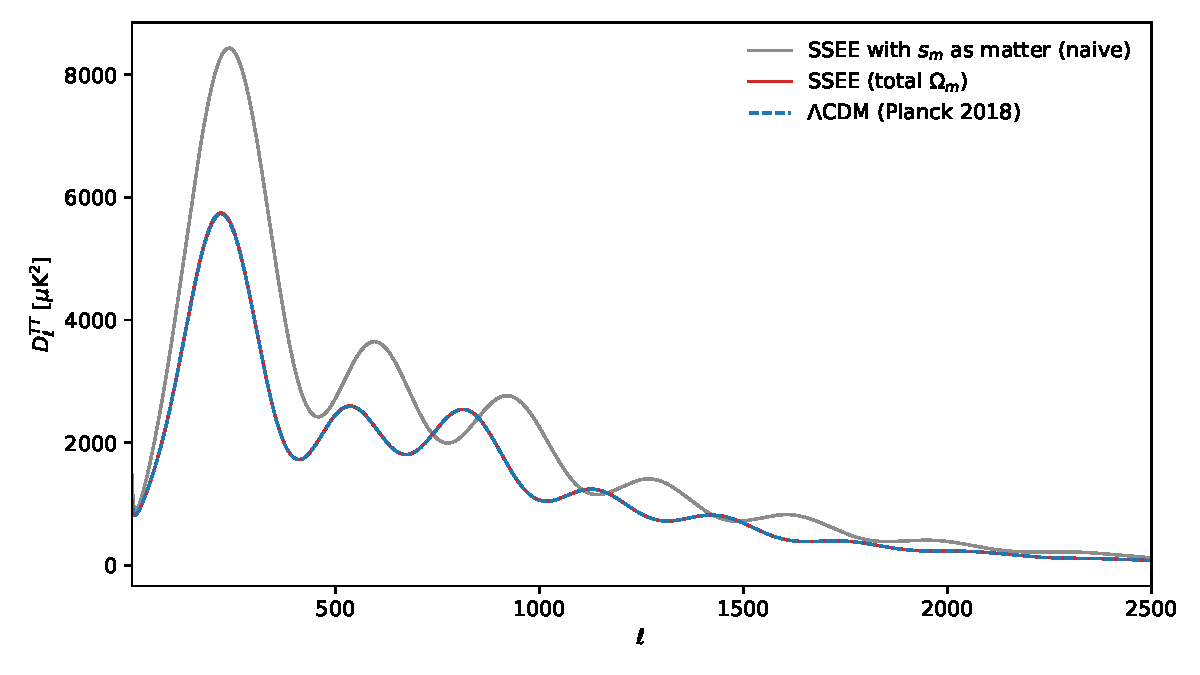
\includegraphics[width=0.82\textwidth]{../results/figures/fig_class_tt.pdf}
\caption{CMB TT power spectrum from CLASS\@. \textit{Blue dashed}: \LCDM\ Planck~2018.
         \textit{Red solid}: SSEE with the full $\omega_m$-direct canonical matter density
         $\OmmCMB=\val{OMEGA_M_TOTAL_d6}$ ($w_0=\val{W0_d6}$, $w_a=\val{WA_d6}$) --- peaks at
         $\ell = \val{cl_ssee_l1}, \val{cl_ssee_l2}, \val{cl_ssee_l3}$, agreeing with \LCDM\ to within $\Delta\ell \le 1$
         (RMS $= \val{cl_ssee_rms}\%$).
         \textit{Grey}: the SSEE dynamical-only run ($\OmmCMB = \val{S_M_d6}$);
         it produces peaks at $\ell = \val{cl_naive_l1}, \val{cl_naive_l2}, \val{cl_naive_l3}$ with RMS $= \val{cl_naive_rms}\%$
         relative to \LCDM, confirming that the \emph{full} matter density
         (not the dynamical $\sm = \val{S_M_d6}$) is needed to reproduce the acoustic scale.}
\label{fig:cmb_tt}
\end{figure}

\subsection{Acoustic-scale mapping and $r_d$}
\label{sec:rd}

The CAMB-based analysis of Paper~3 computes the \SSEE\ drag horizon from the
full $\omega_m$-direct CMB density $\OmmCMB=\val{OMEGA_M_TOTAL_d6}$ (OP-8 dissolved, no matter
factor): the physical drag horizon is
$r_d = 147.17$~Mpc, within $1\sigma$ of the Planck~2018 measurement
$r_d = 147.09\pm0.26$~Mpc \citep{Planck2018} (TT,TE,EE+lowE, Table~2; no BAO prior).
The same full CMB-sector matter density that restores the acoustic peaks
(\S\ref{sec:cmb}) also sets the physical sound horizon; the earlier
interpretation as a $|\wz|$ mapping of the geometric scale is superseded.


% ─────────────────────────────────────────────────────────────────────────────
\section{Structure Growth, $\sigma_8$, and the $f\sigma_8$ Tension}
\label{sec:growth}
% ─────────────────────────────────────────────────────────────────────────────

\subsection{Israel-Stewart causal perturbations: single-sector}
\label{sec:IS}

Because $\wz = \val{W0_d6} < -1/3$, a naive $k$-essence interpretation yields
a bare sound speed $c_{s,\mathrm{bare}}^2 = \wz \simeq -0.840$, implying
catastrophic gradient instability on all sub-horizon scales.
Paper~5 \citep{AlmeidaSSEE2026P5} performs a causal Israel-Stewart (IS)
analysis \citep{IsraelStewart1979} and demonstrates analytically that the
\SSEE\ structure constants satisfy an algebraic identity that forces the
effective IS sound speed to zero:
$c_{s,\mathrm{eff}}^2(k\to\infty) = 0$, to floating-point precision.

Integrating the full IS linear growth ODE from $z=19$ to $z=0$
with $\Omega_{m,\mathrm{cosm}} = \val{OMEGA_M_TOTAL_d6}$ in the Poisson source:
\begin{equation}
  \mathcal{G} = D_1^{\mathrm{SSEE}}/D_1^{\Lambda\mathrm{CDM}} = 1.0032,
  \qquad
  \sigma_8^{\mathrm{SSEE}} = 0.811 \times \mathcal{G} = 0.8136.
  \label{eq:G_IS}
\end{equation}
The IS growth index $\gamma_{\mathrm{IS}} = 0.5504\pm0.001$, consistent with
$\gamma_{\Lambda\mathrm{CDM}} \simeq 0.55$ \citep{Lahav1991}, indicating that
the SSEE perturbation growth rate tracks \LCDM\ at the percent level despite
the different background.

\subsection{The growth amplitude, measured on raw shear data}
\label{sec:growth_raw}

The growth sector has a single matter density, $\Omm=\val{OMEGA_M_TOTAL_d6}$, entering the
background and the growth of structure alike, and it is tested against raw
survey data rather than against compressed statistics whose reduction assumes a
$\Lambda$CDM background.

\paragraph{Cosmic shear.} Against the $357$ unmasked \emph{raw} $\xi_\pm$ points
of \textsc{KiDS-Legacy} (Wright et al.\ 2025, arXiv:2503.19441), with the
background fixed by the algebra and the amplitude free, the shear asks for
$\log(10^{10}A_s)=3.0255\pm0.0396$, $0.49\sigma$ from the $3.04483$ that the
model's own CMB fit supplies. Fixing $A_s$ to that CMB value leaves the growth
sector with \emph{no} free cosmological parameter --- only the eight survey
nuisance parameters --- and costs nothing: $\chi^2_{\rm min}=417.97$ against
$418.34$ with $A_s$ free ($\Delta\mathrm{BIC}=6.24$ in favour of fixing it). The
amplitude is then an output,
\begin{equation}
  S_8 \equiv \sigma_8\sqrt{\Omm/0.3} = 0.8273 ,
  \qquad
  \text{measured } 0.8265\pm0.0176 \;(0.05\sigma),
  \label{eq:s8_raw}
\end{equation}
with no posterior width of its own. KiDS-Legacy predates this analysis by
sixteen months, and no temporal priority is claimed: the result is a
consistency of $A_s$ between the CMB and the growth epoch. The three $\chi^2$
compared (fixed $A_s$, free $A_s$, Planck background) span less than $1.0$, so
cosmic shear does not discriminate between the backgrounds; what separates
them is the parameter count.

\subsection{$f\sigma_8$}
\label{sec:tension_table}

At the single-sector level with the Poisson source at $\OmmCMB=\val{OMEGA_M_TOTAL_d6}$
(Paper~5), the growth factor is $\mathcal{G}=1.0032$ and the mean $\fsig$
tension across six RSD surveys is $0.70\sigma$ --- statistically
indistinguishable from $\Lambda$CDM ($0.73\sigma$). Against the \emph{raw}
BOSS DR12 redshift-space multipoles ($222$ points, one-loop LPT to
$k_{\max}=0.20\,h\,$Mpc$^{-1}$, Alcock--Paczynski applied to the model), the
algebraic background and the Planck background reach $\chi^2=\val{bossR_chi2_ssee}$ and
$\val{bossR_chi2_lcdm}$ with the same $37$ free parameters, each with its own
$\sum m_\nu$: $\Delta\chi^2=\val{bossR_dchi2}$, a mild, not decisive, preference
for the algebraic background (Paper~6).

This analysis operates at the linear-growth level for the growth index;
non-linear effects (baryonic feedback beyond HMcode, halo bias) may modify the
predictions at the $10\%$--$20\%$ level.

% ─────────────────────────────────────────────────────────────────────────────
\section{EFT Stability Analysis}
\label{sec:eft}
% ─────────────────────────────────────────────────────────────────────────────

\subsection{Bellini-Sawicki $\alpha$-functions}
\label{sec:alphas}

Paper~7 \citep{AlmeidaSSEE2026P7} writes the dark-energy sector as a $k$-essence
scalar field with the two-term kinetic function $K(X)=c_1X+c_2X^2$, minimally
coupled to gravity and to matter, with no potential. The ratio
$u\equiv c_2X/c_1=-(M_v+T_r)/(3T_r+M_v)=\val{u_condensado_d6}$ is fixed by the algebraic
equation of state, and reproduces $w_\varphi=\wz=\val{W0_d6}$ exactly. In the
Bellini-Sawicki parametrisation \citep{Bellini2015} this yields
\begin{equation}
  \alphaT = \alphaM = \alphaB = 0 \quad (\text{exact}),
  \qquad
  \alphaK = 3\,\Omega_{\rm DE}\,(5-3\wz) = \val{alpha_K_z0_d6},
  \label{eq:alphas}
\end{equation}
with the dark-energy \emph{density} $\Omega_{\rm DE}=1-\OmmCMB=\val{OMDE_DENS_d6}$.
The vanishing of $\alphaT$, $\alphaM$ and $\alphaB$ implies: (i) gravitational
waves propagate at $c$ (GW170817 compatible at $|\alphaT| < 10^{-15}$
\citep{GW170817,Monitor2017}); (ii) no extra polarisation modes; (iii) standard
light deflection.

\subsection{Stability and what is observable}
\label{sec:eftcamb}

The solution requires $c_1<0$ and $c_2>0$: the field is a ghost condensate,
stabilised at $X/X_{\min}=\val{X_sobre_Xmin_d6}$, where the no-ghost condition
$K_X+2XK_{XX}>0$ holds. Its sound speed is fixed by the same algebra,
\begin{equation}
  c_s^2 = \frac{M_v-T_r}{5M_v+3T_r} = 0.021284 > 0,
  \label{eq:Qs}
\end{equation}
so the sector is gradient-stable. An independent \textsc{hi\_class}
integration reproduces $c_s^2$ to $0.000\%$ and $\alphaK$ to $0.011\%$, with
the internal stability tests enabled (Paper~7). The kineticity itself is
\emph{not} observationally accessible: a factor $100$ change moves $\sigma_8$ by
$0.007\%$ and the TT spectrum only at $\ell<10$, seven times below cosmic
variance. The falsifiable content of this sector is therefore $c_s^2$ and
$\wz$, not $\alphaK$.

The quantity $\val{S_K_d6}$ that appears elsewhere in this journal is not a
kineticity: it is $s_K=-3\wz(1+\wz)=3\,s_{\rm DE}\,s_m$, the fractional
dilution rate of the dark-energy pressure per e-fold, built from the
saturations $s_{\rm DE}=|\wz|=\val{S_DE_d6}$ and $s_m=1+\wz=\val{S_M_d6}$ (numbers of
the equation of state, not densities). It enters $f_{\rm screen}$
(\S\ref{sec:extensions}).

\subsection{CPL phantom crossing and discriminating prediction}
\label{sec:phantom}

When the CPL EoS $w(z) = \wz + \wa z/(1+z)$ is used in the EFTCAMB run,
the phantom boundary $w = -1$ is crossed at $z \simeq 0.31$.
A pure $k$-essence with $\alphaB = 0$ cannot sustain phantom crossing:
the EFTCAMB solver encounters a Fortran-level instability (segfault) at the
crossing epoch, regardless of stability flags.
Earlier versions read this as evidence that completing the SSEE action in the
phantom regime requires $\alphaB \neq 0$, to supply a degree of freedom able
to absorb the null-energy-condition violation.  That reading is superseded,
and the reason is that the phantom regime itself is gone.  In the revised
action of Paper~7 the field is minimally coupled and its equation of state is
constant at $\wz = \val{W0_d6} > -1$: the null energy condition holds at all
times and there is no crossing for $\alphaB$ to absorb.  The phantom crossing
of earlier versions was produced by the conformal dark-sector coupling, which
is withdrawn.

The prediction survives, with its sign reversed and its status improved.
SSEE now predicts $\alphaB = \alphaM = 0$ \emph{exactly and
unconditionally}, so a detection of $\alphaB \neq 0$ above $2\sigma$ by
DESI~Y3 or Euclid ($\sigma \simeq 0.05$) would \emph{falsify} the sector
rather than support it.  What was a discriminating prediction conditional on
a two-sector picture --- an extension withdrawn on 2026-08-01 --- is now an
unconditional one.



% ─────────────────────────────────────────────────────────────────────────────
\section{Extensions: Strong-Field Regime, Hubble Tension, and UV Completion}
\label{sec:extensions}
% ─────────────────────────────────────────────────────────────────────────────

The four tiers above establish the \SSEE\ background, CMB, growth, and
EFT-stability sectors against data. We now summarise three theoretical
extensions, developed in full in Papers~8--10 \citep{AlmeidaSSEE2026P8,
AlmeidaSSEE2026P9,AlmeidaSSEE2026P10}. We label their epistemic status
explicitly: the strong-field lensing signature (\S\ref{sec:ext-sg}) is a
falsifiable prediction; the Hubble-tension screening fraction
(\S\ref{sec:ext-ht}) is a zero-parameter algebraic result compared to existing
data; and the UV completion (\S\ref{sec:ext-uv}) contains one quantity ---
$H_0^{\rm glob,UV} = H_{\rm SH0ES}(1-f_{\rm screen}) = 67.96214$~km\,s$^{-1}$\,Mpc$^{-1}$ (residual $+4.2{\times}10^{-6}$ against the dimensionless target $3(\varphi+\pi)^2$,
not a significance: the propagated uncertainty is $\pm0.968$) --- that is explicitly
conditional on a separability postulate and is therefore presented as a
self-consistency check, not an independent prediction.

\subsection{Strong-field regime: disformal lensing amplification}
\label{sec:ext-sg}

Starting from the $k$-essence action of Paper~7, the disformal coupling between
the dark-energy scalar $\phi$ and dark matter generates deviations from general
relativity (GR) that are algebraically fixed by $\phiG$ and $\pi$. In the
quasi-static limit the scalar field equation closes as a gradient relation,
$\nabla\phi = 2\KAL\,\AURA\,M_{\rm Pl}\,\nabla\Phi_N$, linking the scalar
profile to the Newtonian potential through the structural coupling
$\AURA = (3\phiG+\pi)/2 \approx 3.998$.

From the disformal null geodesic, the total photon deflection angle is amplified
by $\sqrt{\AURA}$ relative to the GR prediction for the same baryonic mass,
giving an algebraic Einstein-radius ratio
\begin{equation}
\left.\frac{\theta_E^{\rm SSEE}}{\theta_E^{\rm GR}}\right|_{\rm alt}
   = \sqrt{\AURA}\approx \val{sqrt_AURA_d4}
   \qquad\text{(alternative MOND-like limit only).}
\end{equation}
The quantity $\sqrt{\AURA}$ is numerically close to $\MIRA=\AURA/2\approx \val{MIRA_d4}$
at $0.03\%$ because $\AURA\approx 4$ makes both round to $2$; the two are
distinct algebraic operations on $\AURA$ and the closeness is not a structural
identity. Solar-system gravitational tests are automatically satisfied: the
disformal coupling selects dark matter as the sole source of $\phi$, so in the
solar system ($\rho_{\rm DM}\approx 0$) the field is locally unsourced and the
disformal metric modification is negligible; equivalently, $K(X)$ is of
$k$-mouflage type \citep{BraxValageas2014} with a screening radius
$r_{\rm km}(\odot)\approx 0.022\,R_\odot$.
\emph{In the canonical limit} --- a single cold matter sector with
$\omega_c = \mathrm{KAL}_0\,\omega_b\,n_s$ (Paper~1, OP-8 closed) plus the
Bellini--Sawicki structure $\alpha_B=\alpha_M=\alpha_T=0$ of Paper~7, which
gives $\mu-1=0$ --- the residual fifth-force is
suppressed to $F_\phi/F_N\sim(H/k)^2\sim 10^{-15}$ at kpc scales and the
canonical observable lensing reduces to $\thetaE^{\rm SSEE}\approx
\thetaE^{\rm GR-with-DM}$. Current SLACS/BELLS samples (mean total slope
$\gamma=2.078\pm 0.027$; $M_E/M_{\rm dyn}\approx 1.21$ for SIS) are consistent
with the canonical limit. A $\sim\MIRA$ matter-power suppression above a $\phi$-DM free-streaming scale
was previously listed here as a falsifiable prediction; it is retracted with the
particle (\S\ref{sec:growth_raw}).

\subsection{The Hubble tension: an algebraic local screening fraction}
\label{sec:ext-ht}

The dark-energy EFT of Paper~7 and the disformal geodesic of Paper~8 together
imply a late-time \emph{local screening fraction}
\begin{equation}
\fscr = \frac{s_K}{3\,\MIRA}
      = \frac{\pi-\phiG}{(\phiG+\pi)^2}
      \approx 0.0673 ,
\end{equation}
where $s_K = -3\wz(1+\wz) = \val{S_K_d6}$ is the pressure dilution rate of
\S\ref{sec:eftcamb} and
$\MIRA = (3\phiG+\pi)/4$. The structural constant $\AURA = 2\MIRA$ cancels
exactly in the ratio, leaving a pure function of $\phiG$ and $\pi$. Applied as a
correction applied to the measured local rate. The only directly measured
expansion rate is the local one, $H_0^{\rm SH0ES}=73.04\pm1.04$
\citep{Riess2022}; Planck's is inferred within $\Lambda$CDM rather than
measured, so SH0ES is the input and the global rate is the output,
\begin{equation}
H_0^{\rm glob,IR} = H_0^{\rm SH0ES}\,(1-\fscr^{\rm IR})
                = 73.04\times(1-0.06725)
                \approx 68.13~{\rm km\,s^{-1}\,Mpc^{-1}} ,
\end{equation}
which lies $0.17\sigma$ from the pure algebraic number
$3(\phiG+\pi)^2=67.96214$ with zero free parameters --- the same number the
$\omega_m$-direct reframe finds preferred by plik\_lite (Paper~3). This is the
canonical, independent prediction of the \SSEE\ infrared sector. (The earlier MIRA anchor
$H_0^{\rm MIRA}=67.037$ gave $71.87$ at $1.12\sigma$, now superseded by the
reframe.) The correction operates at late times
($z<0.15$) through the scalar kinetic-energy contribution to the local expansion
rate; it does not modify the sound horizon $r_d$, the CMB peak positions, or the
growth factor $\sigma_8$ established in the tiers above.

\subsection{UV completion: the \texorpdfstring{$X^2/M^4$}{X2/M4} operator}
\label{sec:ext-uv}

The infrared kinetic Lagrangian $K(X)=X/\KAL$ is extended by the leading
higher-derivative operator, $K(X)=X/\KAL + X^2/M^4$. The inflationary
$\alpha$-attractor parameter $\alpha=\phiG^4/3$ (Paper~1, Appendix~A.5), which
fixes the tensor-to-scalar ratio $r=12\alpha/N_*^2\approx0.00813$, also fixes the
UV cutoff:
\begin{equation}
M^4 = 45\,\alpha^2\,\rho_c = 5\,\phiG^8\,\rho_c \approx 234.9\,\rho_c ,
\qquad M \approx 9.68~{\rm meV} ,
\end{equation}
where the identity $45\alpha^2 = 5\phiG^8$ follows exactly from
$\alpha=\phiG^4/3$. With this cutoff the full Bellini-Sawicki kineticity becomes
$\alphaK^{\rm full}=\val{S_K_FULL_d5}$ ($+3.37\%$ over the IR value). Applied to the
measured SH0ES rate this gives the canonical UV value
$H_0^{\rm glob,UV}=73.04\times(1-\val{F_SCREEN_d6})=67.96214$~km\,s$^{-1}$\,Mpc$^{-1}$ (residual $+4.2{\times}10^{-6}$ against $3(\varphi+\pi)^2$, $\sigma=0.968$;
the earlier MIRA-anchored $72.05$ at $0.96\sigma$ is superseded by the reframe).

We state the epistemic status of these figures plainly: the UV value is
\emph{conditional on Postulate~C.1} (UV--IR $\phiG/\pi$ separability) and is
\emph{not independent of SH0ES}, since the postulate was formulated with the
SH0ES central value as its target. It is a self-consistency check, not a
prediction. The independent prediction remains the IR-regime value
$H_0^{\rm glob,IR}=68.13$~km\,s$^{-1}$\,Mpc$^{-1}$ ($0.17\sigma$) of \S\ref{sec:ext-ht}, which does
not rely on the postulate. The construction does, however, supply a falsifiable
cross-epoch consistency test: the same $\alpha$ governs inflation at $z\sim10^{60}$
and the dark-energy UV scale today, so a LiteBIRD measurement of $r\neq0.00813$
would shift both $\alpha$ and $M$ and change the predicted $H_0^{\rm glob}$
accordingly.

% ─────────────────────────────────────────────────────────────────────────────
\section{Falsifiability and Prediction Register}
\label{sec:falsify}
% ─────────────────────────────────────────────────────────────────────────────

A common objection to algebraically derived frameworks is post-hoc selection:
that combinations of $\phiG$ and $\pi$ are chosen to match known values.
The defence is \emph{structural}, not chronological: the constants are drawn from a
closed dictionary fixed by construction, with no optimisation over formula space.
Table~\ref{tab:register} classifies each derivation by epistemic status. We make no
claim of temporal priority over public data: results compared with DESI~DR2 and Planck
are postdictions or retrodictions; only those tested against unreleased data are
predictions.

\textbf{Global falsification criterion.} The \SSEE framework would be
falsified at the theory level if \textit{any} of the following were established:
(i) $(\wz, \wa)$ is inconsistent with the DESI~DR2 posterior at $>3\sigma$;
(ii) a future CLASS MCMC with Planck+DESI likelihoods requires
$\Omega_{m,\mathrm{CMB}} \neq \val{OMEGA_M_TOTAL_d6}$ at $>3\sigma$;
(iii) cosmic shear places $S_8$ more than $3\sigma$ from $0.8273$ --- the value predicted once $A_s$ is \emph{fixed} to what the CMB gives under the same background, leaving no free cosmological parameter and nowhere to absorb the discrepancy (superseding the weaker earlier form, $3\sigma$ from $0.7555\pm0.0192$ with $A_s$ fitted)
when the primordial amplitude is fitted to raw $\xi_\pm$ data with the \SSEE\
background held fixed;
(iv) $r \neq 0.00813$ as measured by LiteBIRD;
(v) the strong-lensing Einstein-radius ratio is inconsistent with
$\sqrt{\AURA}\approx\MIRA$ at $>3\sigma$ in HST/JWST surveys.

\begin{table}[htbp]
\centering
\caption{Predictive register: \SSEE\ derivations by epistemic status.
         \textit{Postdiction}: algebraic result fixed by the closed dictionary, then
         compared to data already public---no claim of temporal priority.
         \textit{Retrodiction}: derived independently, then compared to existing data.
         \textit{Prediction}: fixed now, tested against not-yet-released data.}
\label{tab:register}
\resizebox{\textwidth}{!}{%
\begin{tabular}{p{6.0cm}lp{4.0cm}l}
\toprule
Quantity (algebraic formula) & Value & Test / Instrument & Status \\
\midrule
\multicolumn{4}{l}{\textit{Background sector (algebraic dictionary)}} \\
$w_0 = -T_r/M_v$ & $\val{W0_d6}$ & DESI DR2 CPL posterior & Postdiction \\
$w_a = -P_{\rm sc}/I_g$ & $\val{WA_d6}$ & DESI DR2 CPL posterior & Postdiction \\
$\MIRA = (3\phiG+\pi)/4$ & $\val{MIRA_d6}$ & $\fscr=\alphaK/(3\MIRA)$ (Papers 8, 9) & Postdiction \\
\midrule
\multicolumn{4}{l}{\textit{Retrodictions (derived independently, compared to existing data)}} \\
$H_0/(\mathrm{km\,s^{-1}\,Mpc^{-1}}) = 3(\phiG+\pi)^2$ & $67.96214$ km/s/Mpc & Planck 2018 & Retrodiction \\
$n_s = 1-\phiG^{-7}$ & $\val{N_S_d6}$ & Planck 2018 & Retrodiction \\
$\OmmCMB = \omega_m/h^2$ ($\omega_m$-direct) & $\val{OMEGA_M_TOTAL_d6}$ & Planck 2018 & Retrodiction \\
$r_d$ (CAMB, $\omega_m$-direct) & $147.17$ Mpc & Planck 2018 $r_d$ ($0.32\sigma$) & Retrodiction \\
$\gamma_{\rm IS} = 0.5504$ & $\approx \gamma_{\Lambda\rm CDM} = 0.55$ & RSD surveys & Retrodiction \\
$\alphaT = \alphaM = \alphaB = 0$ & exact & GW170817 $|\alphaT|<10^{-15}$ & Retrodiction \\
$S_8$ (KiDS-Legacy, $A_s$ fixed by the CMB) & $0.8273$ predicted & measured $0.8265\pm0.0176$ ($0.05\sigma$) & \textbf{Prediction} \\
$S_8$ (MCMC vs.\ raw KiDS-1000 $\xi_\pm$) & $0.7555\pm0.0192$ & $\Lambda$CDM control: $0.7571\pm0.0194$ & Retrodiction \\
$\sigma_8$ ($A_s$ fixed to Planck; ceiling) & $0.8149$ & convention, not a prediction & --- \\
$H_0^{\rm glob,IR} = H_0^{\rm SH0ES}(1-\fscr^{\rm IR})$ & $68.13$ km/s/Mpc & $3(\phiG+\pi)^2=\val{H0_GLOBAL_d5}$ ($0.17\sigma$; IR only, partial) & Retrodiction \\
$H_0^{\rm glob} = H_0^{\rm SH0ES}(1-\fscr^{\rm full})$ & $\val{H0_GLOBAL_d6}$ km/s/Mpc & $3(\phiG+\pi)^2$ (residual $+4.2{\times}10^{-6}$) & Retrodiction \\
\midrule
\multicolumn{4}{l}{\textit{Predictions (not yet observationally accessible)}} \\

$c_s^2 = (M_v-T_r)/(5M_v+3T_r)$ & $0.021284$ & dark-energy clustering (Euclid, LSST) & Prediction \\
$r = \phiG^{-10}$ & $0.008131$ & LiteBIRD $\sim$2032 & Prediction \\
$\theta_E^{\rm SSEE}/\theta_E^{\rm GR}|_{\rm alt} = \sqrt{\AURA}$ & $\val{sqrt_AURA_d4}$ (alt.\ MOND-like limit only) & HST/JWST strong lensing & Conditional prediction (not canonical; OP-13) \\
\bottomrule
\end{tabular}%
}
\end{table}


% ─────────────────────────────────────────────────────────────────────────────
\section{Discussion and Outstanding Challenges}
\label{sec:discussion}
% ─────────────────────────────────────────────────────────────────────────────

The consolidated results show that \SSEE\ is consistent with four independent
observational tests without adjusting any algebraic parameter.
The most significant open challenges are:

\textbf{(i) $\omega_m$-direct residual dependencies.}
The CLASS tests confirm that the full $\omega_m$-direct density
$\OmmCMB = \omega_m/h^2 = \val{OMEGA_M_TOTAL_d6}$ (built from $\omega_b+\omega_c+\omega_\nu$,
no matter factor; OP-8 dissolved) is physically necessary for CMB peak
reproduction, and it is \emph{not} a free knob: $\omega_c = \mathrm{KAL_0}\cdot\omega_b\cdot n_s$
is a forward algebraic identity (Paper~1). The honest residual is that $\OmmCMB$
now rests on $\omega_b$ (OP-1, partially resolved: the algebraic form is fixed,
the BBN chain is not) and this $\omega_c$ identity being
correct---a dependency chain, not an undetermined parameter.

\textbf{(ii) $S_8$ at the non-linear level.}
The growth amplitude is fixed by the CMB and predicts $S_8=0.8273$ against
raw KiDS-Legacy (\S\ref{sec:growth_raw}). The open item is a precision
question: a full N-body treatment of baryonic feedback (deferred for
computational cost) is required to confirm the linear-theory $S_8$ at the
non-linear level.

\textbf{(iii) Quantum field theory completion.}
The algebraic connection $H_0/(\mathrm{km\,s^{-1}\,Mpc^{-1}}) = 3(\phiG+\pi)^2$ is a successful numerical
retrodiction but lacks a derivation from first-principles quantum field theory.
Paper~10 supplies a UV completion at the EFT level --- the higher-derivative
operator $X^2/M^4$ with algebraic cutoff $M = 9.68$~meV --- but a derivation of
the full $P(X,\phi)$ Lagrangian from $\phiG$ and $\pi$ alone remains open.
Under the $\omega_m$-direct reframe (OP-8 dissolved) the CMB matter density is
the standard $\Omega_{m,\mathrm{CMB}} = \omega_m/h^2 = \val{OMEGA_M_TOTAL_d6}$, with no matter
factor; the earlier MIRA-mapped $0.31993$ and geometric
$(\pi-\phiG)/(\pi+\phiG)=0.32010$ forms are superseded. The residual open
problem is now only the UV origin of the algebraic $\omega_c=\mathrm{KAL_0}\,\omega_b\,n_s$
identity.


% ─────────────────────────────────────────────────────────────────────────────
\section{Conclusions}
\label{sec:conclusions}
% ─────────────────────────────────────────────────────────────────────────────

We have presented a consolidated validation of the \SSEE framework
across four observational tiers.

\begin{enumerate}[leftmargin=*,itemsep=2pt]
\item \textbf{Background sector.} The algebraic prediction
  $(\wz, \wa) = (-0.840, -0.670)$, fixed by construction (not fitted), lies within
  $0.24\sigma$ of the official DESI~DR2 $w_0w_a$CDM posterior (Pantheon+).
  A Bayesian MCMC yields
  $H_0 = 67.82\pm0.41$~km\,s$^{-1}$\,Mpc$^{-1}$ under $H_0^{\rm glob}$
  as prior ($0.33\sigma$ from it), and $\Delta\mathrm{BIC} = \val{p2_dBIC_lcdm}$ favouring \SSEE\ over \LCDM.
  A complementary full-likelihood multi-probe MCMC ($w_0,w_a$ free, $H_0$
  free under the uncompressed CMB likelihood) recovers the CMB combinations
  $\omega_b,\omega_c,r_{\rm drag}$ to $\le0.2\sigma$ and places \SSEE\ at
  $1.31\sigma$ in the $w_0$--$w_a$ plane, where \LCDM\ is excluded at $3.22\sigma$.

\item \textbf{CMB Boltzmann.} CLASS confirms that the full $\omega_m$-direct
  matter density ($\OmmCMB=\val{OMEGA_M_TOTAL_d6}$) is physically necessary: with only the
  dynamical $\sm=\val{S_M_d6}$, the CMB RMS residual jumps by a factor of \val{cl_degrada} and
  all three acoustic peaks shift by $\sim 10\%$.
  With the full $\omega_m$-direct density, peak positions agree with \LCDM\ to
  within $\Delta\ell \le 1$ (RMS $= \val{cl_ssee_rms}\%$).

\item \textbf{Structure growth.} The IS perturbation analysis
  ($\OmmCMB=\val{OMEGA_M_TOTAL_d6}$ in Poisson) gives $\mathcal{G} = 1.0032$ and $\sigma_8 = 0.8136$,
  with mean $f\sigma_8$ tension $0.70\sigma$ (Paper~5) --- statistically identical
  to $\Lambda$CDM ($0.73\sigma$). In the lensing amplitude, with $A_s$ fixed to the
  value the model's own CMB fit supplies and no free cosmological parameter,
  a single matter sector predicts $S_8=0.8273$ against $0.8265\pm0.0176$ from
  raw KiDS-Legacy $\xi_\pm$ (Paper~6). Against raw BOSS DR12 multipoles the
  algebraic background fits marginally better ($\chi^2=\val{bossR_chi2_ssee}$ vs $\val{bossR_chi2_lcdm}$, same
  freedom).

\item \textbf{EFT stability.} The two-term $k$-essence of Paper~7 is a ghost
  condensate, ghost-free and gradient-stable with $c_s^2 = 0.021284$;
  $\alphaT = \alphaM = \alphaB = 0$ exactly (GW170817 compatible) and
  $\alphaK = \val{alpha_K_z0_d6}$, which is not observationally accessible. A detection of
  $\alphaB \neq 0$ would falsify the sector. The same action fixes $\wz$ but
  does not produce $\wa$ (OP-24).

\item \textbf{Theoretical extensions.} The disformal strong-field regime predicts
  an Einstein-radius amplification $\sqrt{\AURA}\approx\MIRA$, falsifiable with
  HST/JWST strong lensing (Paper~8). An algebraic late-time screening fraction
  $\fscr^{\rm IR}=(\pi-\phiG)/(\phiG+\pi)^2\approx0.067$ takes the measured SH0ES
  rate as input and returns the global background
  $H_0^{\rm glob,IR}=H_0^{\rm SH0ES}(1-\fscr^{\rm IR})=68.13$~km\,s$^{-1}$\,Mpc$^{-1}$,
  $0.17\sigma$ from the pure number $3(\phiG+\pi)^2=\val{H0_ALG_d5}$, with
  zero free parameters (Paper~9). A UV completion $K(X)=X/\KAL+X^2/M^4$ with
  algebraic cutoff $M=9.68$~meV connects the dark-energy EFT to the inflationary
  $\alpha$-attractor; the associated $H_0^{\rm glob,UV}=\val{H0_GLOBAL_d5}$~km\,s$^{-1}$\,Mpc$^{-1}$
  ($4.3{\times}10^{-6}\sigma$ from $3(\varphi+\pi)^2$; the earlier MIRA-anchored $72.05$ at $0.96\sigma$ is superseded)
  is a self-consistency check conditional on a separability postulate, not an
  independent prediction (Paper~10).
\end{enumerate}

The framework generates four near-term falsifiable predictions, under the stated
assumptions (a fifth, a $\phi$-DM free-streaming scale in $P(k)$, is withdrawn
with the particle; \S\ref{sec:growth_raw}): the dark-energy sound speed $c_s^2 = 0.021284$, $\alphaB = 0$ (a detection
would falsify the sector), $r = 0.008131$ (LiteBIRD), and $S_8 = 0.8273$ with no
free cosmological parameter (Paper~6).
All analytical scripts, CLASS configuration files, and EFTCAMB inputs are archived
at Zenodo \citep{AlmeidaSSEE2026zenodo}.

% ─────────────────────────────────────────────────────────────────────────────
\appendix
\section{Complete Algebraic Parameter Table}
\label{app:params}
% ─────────────────────────────────────────────────────────────────────────────

\begin{table}[htbp]
\centering
\caption{Complete set of \SSEE algebraic parameters. All values are
         derived from $\phiG = (1+\sqrt{5})/2$ and $\pi$; no fitting was
         performed. Planck 2018 values \citep{Planck2018} and DESI~DR2
         \citep{AbdulKarim2025} listed for comparison where applicable.}
\label{tab:params}
\resizebox{\textwidth}{!}{%
\begin{tabular}{ll p{0.18\textwidth} p{0.35\textwidth}}
\toprule
Parameter & Formula & SSEE value & Observed \\
\midrule
$w_0$ & $-T_r/M_v = -(3\phiG+\pi)/[2(\phiG+\pi)]$ & $\val{W0_d6}$ & $-0.838\pm0.057$ (DESI) \\
$w_a$ & $-P_{\rm sc}/I_g$ & $\val{WA_d6}$ & $-0.631\pm0.226$ (DESI) \\
$H_0$ & $3(\phiG+\pi)^2$ & $67.96214$ km/s/Mpc & $67.36\pm0.54$ (Planck) \\
$n_s$ & $1-\phiG^{-7}$ & $\val{N_S_d6}$ & $0.9649\pm0.0042$ (Planck) \\
$\OmmCMB$ & $\omega_m/h^2$ ($\omega_m$-direct) & $\val{OMEGA_M_TOTAL_d6}$ & $0.3153\pm0.0073$ (Planck) \\
$\Omde$ & $1-\OmmCMB$ (density) & $\val{OMDE_DENS_d6}$ & $0.6847$ (\LCDM) \\
$s_{\rm DE}$ & $T_r/M_v = |w_0|$ (saturation, not a density) & $\val{S_DE_d6}$ & --- \\
$\sm$ & $1 - s_{\rm DE} = 1+w_0$ (saturation, not a density) & $\val{S_M_d6}$ & --- \\
$\MIRA$ & $(3\phiG+\pi)/4$ (Mirror Ratio; enters $\fscr$) & $\val{MIRA_d6}$ & --- \\
\midrule
$\KAL$ & $\beta + \pi = (\phiG+3\pi)/2$ & $\val{KAL0_d6}$ & --- \\
$\alphaK$ & $3\,\Omde(5-3w_0)$ & $\val{alpha_K_z0_d6}$ & not accessible \\
$s_K$ & $-3w_0(1+w_0)$ & $\val{S_K_d6}$ & --- (enters $\fscr$) \\
$c_s^2$ & $(M_v-T_r)/(5M_v+3T_r)$ & $0.021284$ & --- \\
$\alphaT = \alphaM = \alphaB$ & minimal coupling & $0$ & $|\alphaT|<10^{-15}$ (GW170817) \\
\midrule
$S_8$ & KiDS-Legacy, $A_s$ fixed by the CMB & $0.8273$ predicted & $0.8265\pm0.0176$ (KiDS-Legacy) \\
$S_8$ & MCMC vs.\ raw KiDS-1000 $\xi_\pm$ & $0.7555\pm0.0192$ & $0.759\pm0.024$ (KiDS-1000) \\
$r$ & $\phiG^{-10}$ & $0.008131$ & $<0.036$ (BK18) \\
\midrule
$\fscr$ & $(\pi-\phiG)/(\phiG+\pi)^2$ & $0.0673$ & --- \\
$H_0^{\rm glob}$ & $H_0^{\rm SH0ES}(1-\fscr^{\rm full})$ & $\val{H0_GLOBAL_d6}$ km/s/Mpc & $3(\phiG+\pi)^2$, residual $+4.2{\times}10^{-6}$ \\
$M$ (UV cutoff) & $(5\phiG^8\rho_c)^{1/4}$ & $9.68$ meV & --- \\
\bottomrule
\end{tabular}%
}
\end{table}

% ─────────────────────────────────────────────────────────────────────────────
% ----------------------------------------------------------------------------
\section*{Acknowledgments}
The author acknowledges the use of the cosmological codes \textsc{class} \citep{Blas2011}, \textsc{eftcamb} \citep{Hu2014}, and the Markov Chain Monte Carlo sampler \textsc{Cobaya} \citep{Torrado2021} for the numerical validation of the SSEE framework. The author also acknowledges the use of the \textsc{GetDist} package \citep{Lewis2019} for the analysis and plotting of posterior distributions.

\section*{Data and Code Availability}
The \SSEE\ framework is fully transparent and reproducible. All DESI~DR2 BAO data used in this analysis are publicly available at \url{https://data.desi.lbl.gov/}, and the Planck~2018 cosmological parameter chains at the Planck Legacy Archive (\url{https://pla.esac.esa.int/}). The complete code repository --- including the \textsc{class} and \textsc{eftcamb} configuration files, the \textsc{Cobaya} MCMC chains, the explicit record of Open Theoretical Problems (OP), and the cosmological validation ledgers --- is publicly available at the GitHub repository \url{https://github.com/mikealmeida1721/SSEE-Cosmologia} and archived at Zenodo: \url{https://doi.org/10.5281/zenodo.20093447}.

\clearpage
\bibliographystyle{plainnat}
\bibliography{ssee_unified}
% ─────────────────────────────────────────────────────────────────────────────

\end{document}
